\section{PROTÓTIPOS DE TELA}
\label{sec:titSecPrototipos}

% Os protótipos de tela são uma versão inicial de um sistema. Eles são usados, dentre outras razões, para descobrir mais sobre um problema e suas possíveis soluções. O desenvolvimento rápido e iterativo do protótipo previne gastos desnecessários e custos controlados e os \textit{stakeholders} podem fazer usos pontuais de partes do sistema desde o início do desenvolvimento \citeonline{Sommerville10}.

% Além disso, os protótipos podem ajudar na antecipação de mudanças que podem ser requisitadas.
% Para o presente projeto foram desenvolvidas três interfaces para dois tamanhos diferentes de tela, simulando um dispositivo de tela maior (\textit{desktop}, \textit{tablet}) e outro para telas menores (\textit{smartphones}).

% O modelo de prototipação é ideal quando o cliente não tem os requisitos muito bem definidos, que é o caso do aplicativo estudado neste documento. Visto que os requisitos foram levantados com base em uma planilha, conforme explicado anteriormente na \autoref{sub:processo}.

Nas próximas subseções serão exibidos os protótipos de tela para três principais operações que o usuário poderá realizar no sistema, que são a tela que o usuário é enviado após fazer o \textit{login}, a tela para criação de um novo recurso no sistema e a tela de exibição de um recurso.

\subsection{Protótipos para tela inicial do sistema}
\label{sec:titSecPrototiposHome}

As Figuras \ref{fig:prototipo_home_desk} e \ref{fig:prototipo_home_mobile}, representam a visão da página inicial do sistema, que será exibida após o login do usuário. É possível observar que logo na parte superior, existirão quadros informativos sobre a quantidade de propriedades assistidas, quantidade de cidades atendidas e a área em hectares que foram tratadas (ou corrigidas). Logo abaixo serão exibidas as últimas correções realizadas pelo usuário.

\begin{figure}[H]
    \centering
    \caption{Página que será exibida após o login do usuário na visão de um dispositivo \textit{desktop}}
    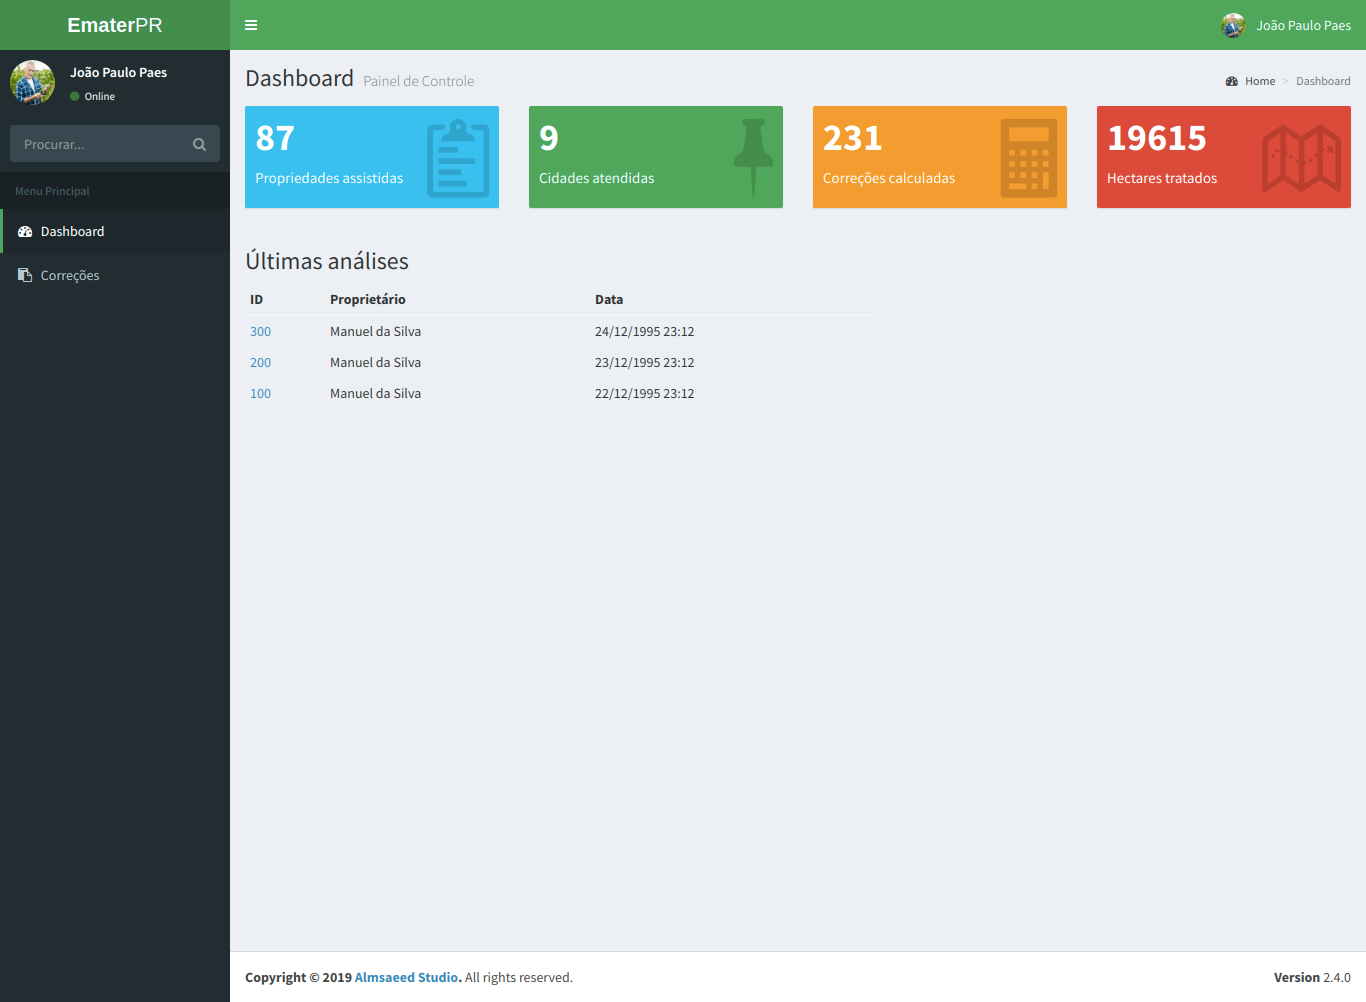
\includegraphics[width=13cm]{./dados/figuras/prototipos/home_desktop.png}
    \label{fig:prototipo_home_desk}
    \fonte{Autoria própria}
\end{figure}

\begin{figure}[H]
    \centering
    \caption{Página que será exibida após o login do usuário na visão de um dispositivo \textit{mobile}}
    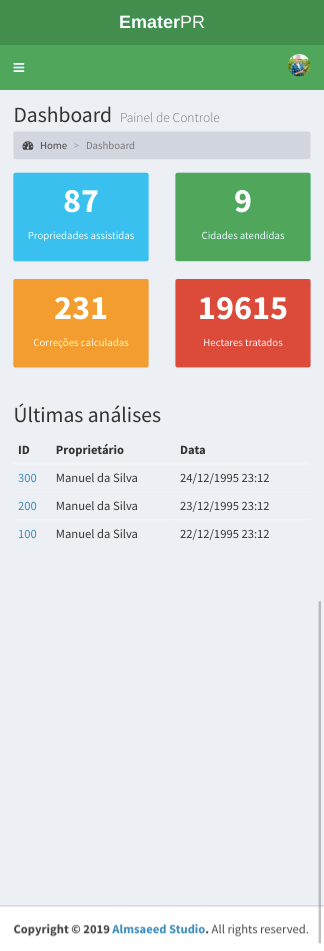
\includegraphics[width=6cm]{./dados/figuras/prototipos/home_mobile.png}
    \label{fig:prototipo_home_mobile}
    \fonte{Autoria própria}
\end{figure}

\subsection{Protótipos para tela de cadastro de informação}
\label{sec:titSecPrototiposCreate}

A tela de cadastro de informações foi pensada para ser intuitiva e reativa como a planilha. Como é um formulário grande, será divido em \textit{steps} que serão exibidos na parte superior do formulário, tendo a descrição do que deve ser feito naquele \textit{step} logo abaixo. Já o formulário propriamente dito terá uma interface reativa, que lembra a planilha.

No exemplo mostrado nas Figuras \ref{fig:prototipo_create_desk} e \ref{fig:prototipo_create_mobile}, é possível observar que caso o valor de um campo esteja no intervalo ideal, este deverá ter a sua \textit{label} e o contorno destacados em verde. Enquanto se o valor estiver fora do intervalo, em âmbar. 

\begin{figure}[H]
    \centering
    \caption{Criação de recurso na visão de um dispositivo \textit{desktop}}
    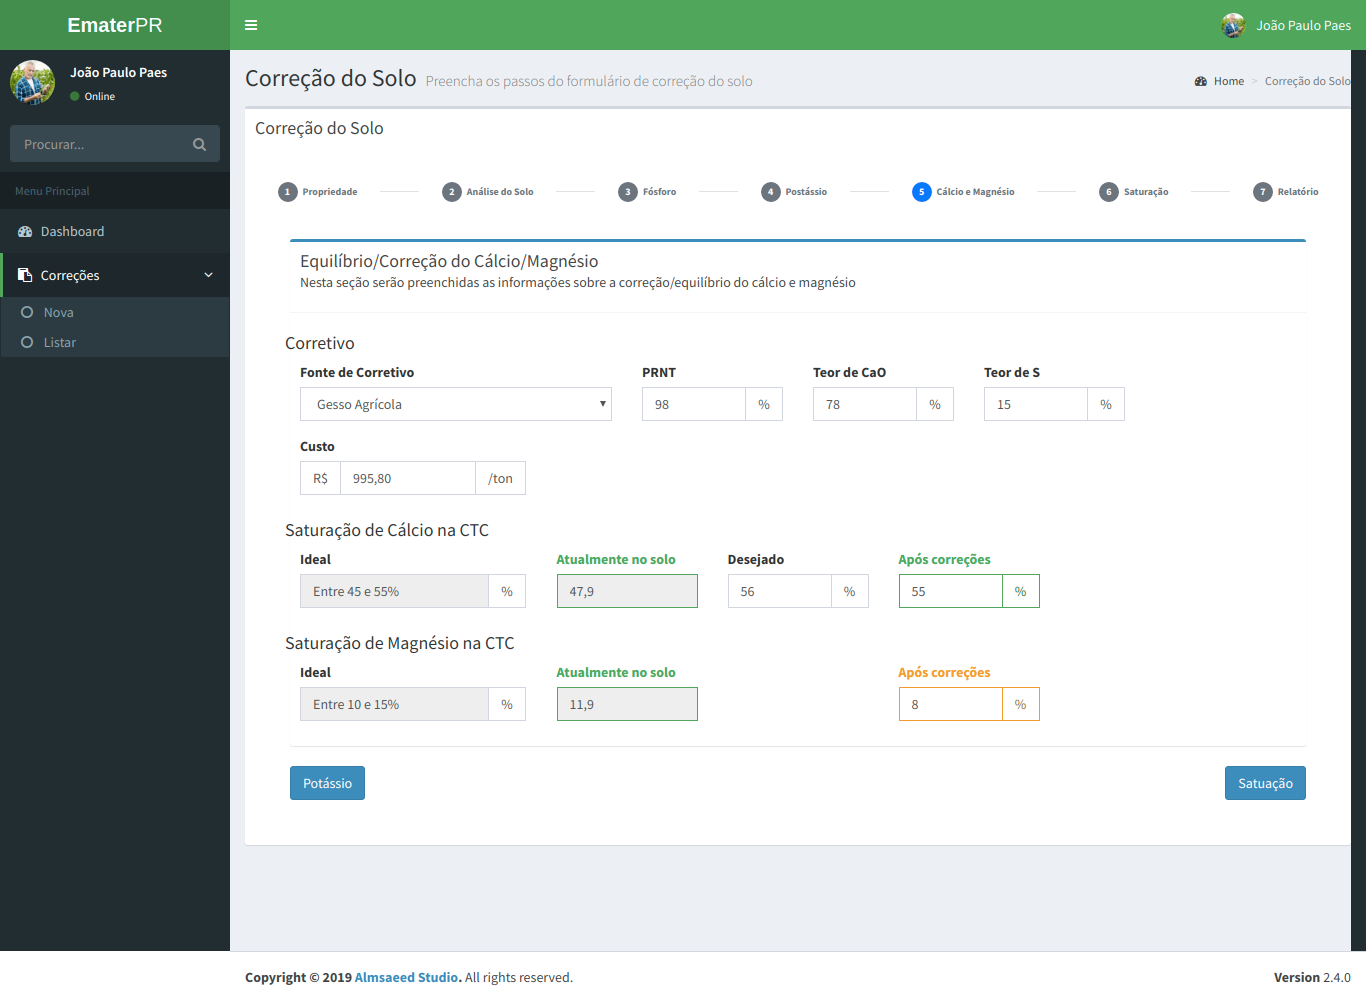
\includegraphics[width=13cm]{./dados/figuras/prototipos/create_desktop.png}
    \label{fig:prototipo_create_desk}
    \fonte{Autoria própria}
\end{figure}

\begin{figure}[H]
    \centering
    \caption{Criação de recurso na visão de um dispositivo \textit{mobile}}
    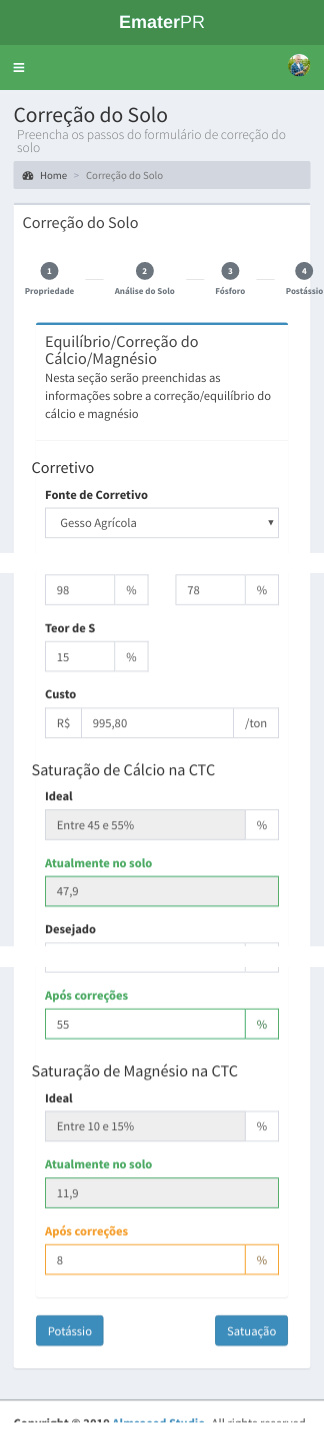
\includegraphics[width=6cm]{./dados/figuras/prototipos/create_mobile.png}
    \label{fig:prototipo_create_mobile}
    \fonte{Autoria própria}
\end{figure}


\subsection{Protótipos para tela de exibição de informação}
\label{sec:titSecPrototiposShow}

A tela de exibição da informação também seguirá o modelo de \textit{steps}. Ela deverá ser dividia em 3 colunas para representar os três estados da correção do solo: naquele momento, desejado e após as correções. É possível notar que os textos deverão estar coloridos de acordo com o caso no qual se encaixa. Acima do valor, amarelo. Abaixo do valor, vermelho. No intervalo, verde.

\begin{figure}[H]
    \centering
    \caption{Visualização de recurso na visão de um dispositivo \textit{desktop}}
    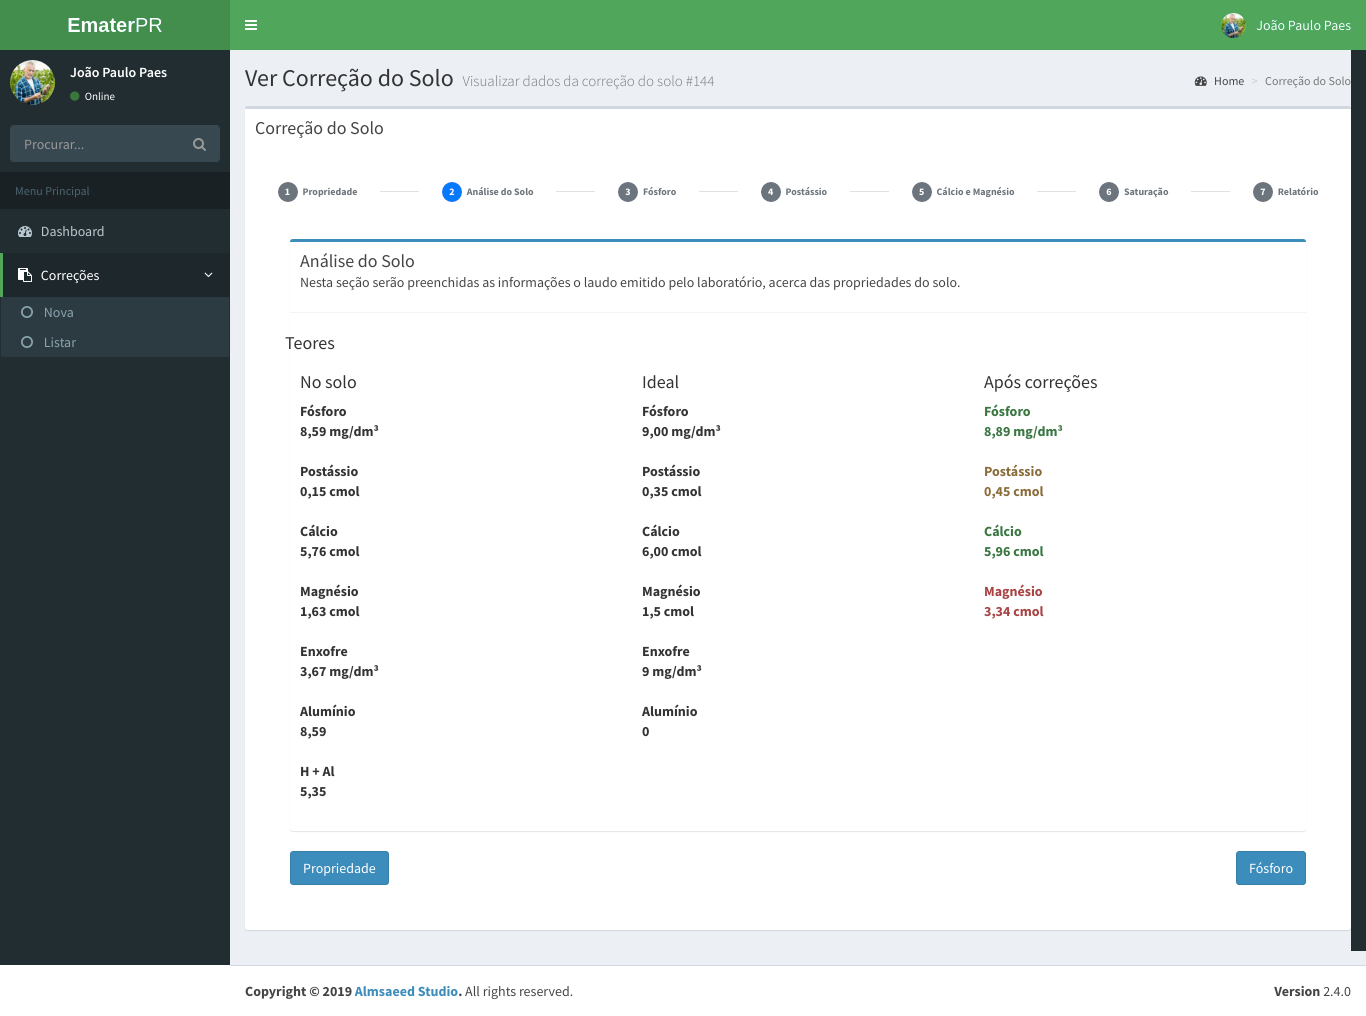
\includegraphics[width=13cm]{./dados/figuras/prototipos/show_desktop.png}
    \label{fig:prototipo_show_desk}
    \fonte{Autoria própria}
\end{figure}

\begin{figure}[H]
    \centering
    \caption{Visualização de recurso na visão de um dispositivo \textit{mobile}}
    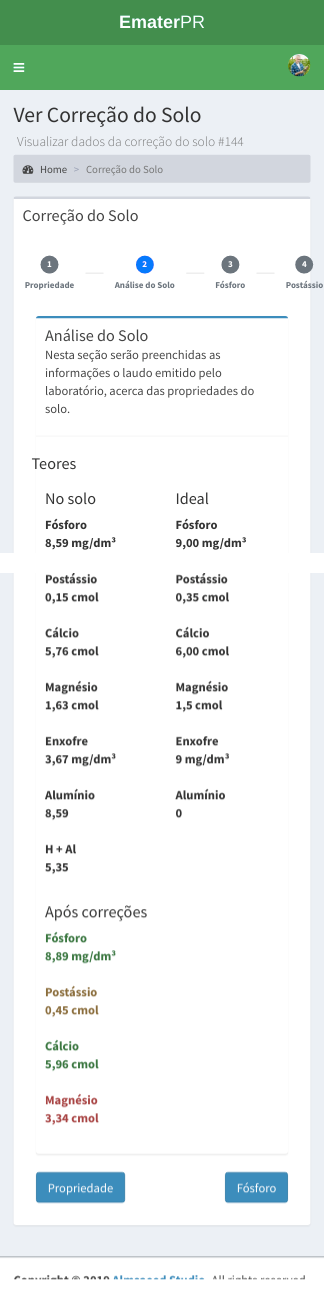
\includegraphics[width=6cm]{./dados/figuras/prototipos/show_mobile.png}
    \label{fig:prototipo_show_mobile}
    \fonte{Autoria própria}
\end{figure}